\documentclass[a4paper, 10pt, notitlepage]{article}

\usepackage{moreverb} %para importar codigo

\usepackage[spanish,activeacute]{babel}
\usepackage{babel} %paquete de idioma

\usepackage[latin1]{inputenc}

\usepackage{pepotina} %caratula
%\usepackage{color}

%\usepackage{hyperref}
%\usepackage[all]{hypcap}

\usepackage{fancyhdr} %linea sup con comentarios

\usepackage{lscape} %para hoja apaisada

\usepackage{framed} %para crear cajas de texto

\usepackage{lastpage} %ultima pagina

%\usepackage{wrapfig} %Inclusi�n de gr�ficos al lado de texto
%\usepackage[rflt]{floatflt} %Para meter figuras flotantes entre el texto


%\usepackage{pstricks}
%\usepackage{uml} %UML

\usepackage{listings}
%\lstset{
%  breaklines=true,                                     % line wrapping on
%  language=ocl,
%  frame=ltrb,
%  framesep=5pt,
%  basicstyle=\normalsize,
%  keywordstyle=\ttfamily\color{OliveGreen},
%  identifierstyle=\ttfamily\color{CadetBlue}\bfseries,
%  commentstyle=\color{Brown},
%  stringstyle=\ttfamily,
%  showstringspaces=ture
%}

\addtolength{\topmargin}{-50pt} 
\addtolength{\textwidth}{105pt}
\addtolength{\textheight}{120pt}
\addtolength{\oddsidemargin}{-50pt}

%\newcommand{\minix}{\textsl{minix }}

%%% Encabezado y pie de p'agina
\pagestyle{fancy}
\fancyhead[LO]{Sistemas Operativos}
\fancyhead[C]{}
\fancyhead[RO]{P\'agina \thepage\ de \pageref{LastPage}}
\renewcommand{\headrulewidth}{0.4pt}
\fancyfoot{}

\newcommand{\depto}{{\bf DPTO: }}


\def\falta#1{ \begin{framed}	\begin{center} \hspace{1cm} \Large FALTA \normalsize #1 \hspace{1cm} \end{center} \end{framed}}


\def\imagen#1#2{\vskip0.5cm
\begin{center}
\includegraphics[scale=#1]{#2}
\end{center}}


\begin{document}

\universidad{Universidad de Buenos Aires}
\facultad{Facultad de Ciencias Exactas y Naturales}
\departamento{Departamento de Computaci�n}
\materia{Sistemas Operativos}
\resumen{Simusched}
\keys{Scheduling, c++, FCFS}
\titulo{Tp1: Simusched}
\subtitulo{Scheduling de tareas}
\grupo{Numero de grupo: 12}
\fecha{1er Cuatrimeste 2011}
\footspace{1cm}
\integrante{Dominguez, Pablo Sebastian}{108/05}{pablo.sebastian.dominguez@gmail.com}
\integrante{Engler, Christian Alejandro}{314/05}{caeycae@gmail.com}

%caratula	
\maketitle{}

\tableofcontents

\newpage



\part{Entendiendo el Simulador simusched}

\section{Ejercicio 1}

Implementamos el m\'etodo TaskCon que simula ser una tarea interactiva, que recibe los par\'ametros \verb|n|, \verb|bmin| y \verb|bmax|.

Realiza \verb|n| llamadas bloqueantes de duraci\'on entre \verb|bmin| y \verb|bmax|.

\begin{framed}
\begin{verbatimtab}
void TaskCon(vector<int> params) { // params: 3
	int n = params[0];
	int bmin = params[1];
	int bmax = params[2];
	
	for( int i = 0; i < n ; i++ ) {
		int time = bmin;
		if(bmin != bmax)
			time = (rand()%(bmax-bmin+1))+bmin;
		uso_IO(time);
	}
}
\end{verbatimtab}
\end{framed}

\section{Ejercicio 2}

Escribimos un lote de 3 tareas distintas: una intensiva en CPU y las otras dos de tipo interactivo. 
El lote lo escribimos en \verb|ejercicio2.tsk|.

\begin{framed}
\begin{verbatim}
# FILE ejercicio2.tsk
TaskCPU 10
@1
TaskCon 10 1 4
@3
TaskCon 7 1 3
\end{verbatim}
\end{framed}

Luego ejecutamos Simusched con Scheduler FCFS con los siguientes parametros:

\begin{verbatim}
./simusched ejercicio2.tsk 1 SchedFCFS | python graphsched.py > ejercicio2.png
\end{verbatim}

Y obtuvimos el siguiente diagrama de Gantt.

\begin{figure}[H]
  \centering
    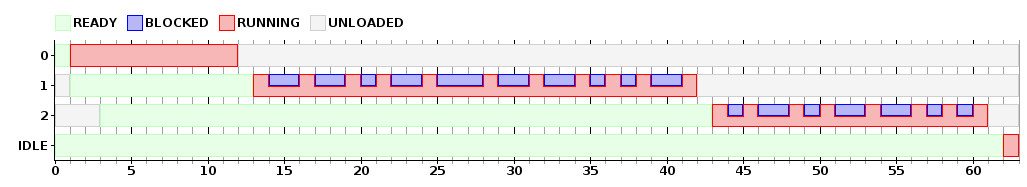
\includegraphics[width=1\textwidth]{img/ejercicio2.png}
    \caption{Una tarea de uso intensivo del procesador y dos interactivas con Scheduling FCFS.}
\end{figure}

Se ve en el diagrama que las tareas se ejecutan en el orden de llegada y que al no existir desalojo en FCFS las tareas mantienen el procesador incluso al estar bloqueadas.


\newpage
\section{Otras modificaciones}

Ahora como el server es multithread cuando el cliente finaliza su conexi\'on con el servidor, tanto por una falla como por decisi\'on propia, no debe finalizar el juego. Para lo cual modificamos el ciclo de cada thread que ante la finalizaci\'on solamente corta el thread de ese jugador.

Dado el comportamiento que le estamos dando al juego con esta modificaci\'on, el backend ahora no finaliza, este se queda escuchando constantemente el ingreso o egreso de clientes.

-//TODO Ver cuando liberar los mutex.
\newpage
\part{Evaluando los algoritmos de scheduling}

\section{Ejercicio 6}

Implementamos el tipo de tarea TaskBatch que recibe como par\'ametro \verb|tot| (tiempo total de ejecuci\'on) y \verb|blocks| (cantidad de bloqueos).

\begin{framed}
\begin{verbatimtab}
void TaskBatch(vector<int> params) {
	int tot = params[0];
	int blocksC = params[1];
	
	vector<bool> blocks = vector<bool>(tot-1);
	for(int i=0;i<blocksC;i++) {
		int blockT = rand()%(blocks.size()-1);
		if( !blocks[blockT] )
			blocks[blockT] = true;
		else
			i--;
	}
	for(int i=0;i<(int)blocks.size();i++) {
		if( blocks[i] )
			uso_IO(1);
		else
			uso_CPU(1);
	}
}
\end{verbatimtab}
\end{framed}

\section{Ejercicio 7}

Primero pensamos que medidas afectar\'ian a un scheduler que procese tareas de tipo Batch.

\begin{description}
 \item[Eficiencia] tratar de que la CPU este ``ocupada'' todo el tiempo.
 \item[Turnaround] tiempo total desde que se carga el proceso hasta que finaliza.
 \item[Latencia] tiempo requerido para que un proceso empiece a dar resultados.
 \item[Waiting Time] tiempo de espera de un proceso en la cola de listos.
\end{description}

Una vez establecidas las medidas que nos interesaban optimizar, tomamos el siguiente lote de tareas para ejecutar.

\begin{framed}
\begin{verbatimtab}
# FILE ejercicio7.tsk
TaskBatch	 	30  1  # p0
TaskBatch	 	30  3  # p1
TaskBatch	 	30  5  # p2
TaskBatch	 	30 10  # p3
TaskBatch	 	30 20  # p4
\end{verbatimtab}
\end{framed}

Para medir los distintos aspectos a optimizar, desarrollamos una clase en java \verb|SchedRRTest.java| que hiciera este trabajo autom\'aticamente.\\
Nota: compilar con \verb|make SchedRRTest| (no lo agregamos en el \verb|make| general en caso de que no tengan instalado el compilador de java)

Esta clase toma como input la salida del \verb|simusched| y retorna por stdout los siguientes valores:

\begin{verbatim}
IDLE <tiempo idle> <datos proc_1> <datos proc_2> ... <datos proc_N>
donde <datos proc_i> es
[<turnaround> <latencia> <waitingTime> <tiempoEntreIOs>]
\end{verbatim}

Creamos el siguiente sh para lanzar autom\'aticamente la ejecuci\'on del \verb|simusched| con distintos valores de quantum. Adem\'as realiza los gr\'aficos de scheduling y las mediciones con nuestro programa SchedRRTest.

\begin{framed}
\begin{verbatim}
rm -f SchedRRTest.count
for i in 1 5 10 15 20 25 30 35
do
        eval png=SchedRRTest$i.png
        eval out=SchedRRTest$i.out
        ./simusched ejercicio7.tsk 1 SchedRR $i > $out
        tail -n 1000 $out | java SchedRRTest >> SchedRRTest.count
        tail -n 1000 $out | python graphsched.py > $png
done
\end{verbatim}
\end{framed}

Utilizando los resultados de la clase SchedRRTest generamos los siguientes gr\'aficos. Estos muestran en el eje \verb|x| los valores de quantum y en el eje \verb|y| el tiempo.

\subsection{Turnaround y Waiting Time}
\begin{figure}[H]
  \centering
    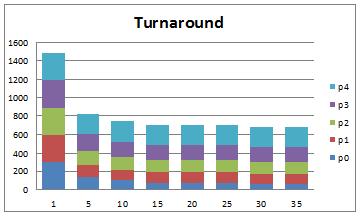
\includegraphics{img/turnaround.png}
    \caption{Gr\'afico comparativo de Turnaround para distintos quantums.}
\end{figure}

\begin{figure}[H]
  \centering
    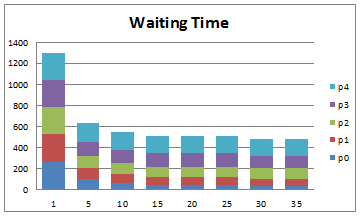
\includegraphics{img/waitingTime.png}
    \caption{Gr\'afico comparativo de Waiting Time para distintos quantums.}
\end{figure}

Se puede observar que los tiempo de \ta y \wt para los procesos con valores de \quantum entre 1 y 5 toman valores muy grandes. Esto se debe a que se producen muchos \cs, donde cada uno aporta 1 ciclo. Esto va a dejar de influir a medida que el \quantum se hace m\'as grande.
Lo que podemos notar adem\'as es que a medida que el \quantum aumenta los tiempos de \ta y \wt disminuyen, aunque no de una manera considerable a partir de valores de \quantum mayores a 15.

\subsection{Latencia}

\begin{figure}[H]
  \centering
    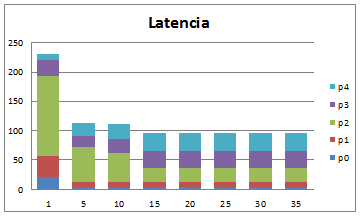
\includegraphics{img/latencia.png}
    \caption{Gr\'afico comparativo de Latencia para distintos quantums.}
\end{figure}

Se puede observar que el tiempo de latencia para los procesos con valor de quantum 1 toma valores muy grandes. Esto se debe a que se ira intercambiando entre los distintos procesos y en promedio se tardar\'a m\'as tiempo en llegar a producirse un primer resultado (IO). 

Para que la latencia sea \'optima, deber\'ia ejecutarse cada proceso hasta que alcance su primer IO. Esto se alcanza al aumentar el \quantum lo suficiente para alcanzar el primer IO de cada proceso. Esto se logra a partir del \quantum 15. Por m\'as que se aumente el \quantum no vamos a mejorar la \latencia


Para ver esto veamos los gr\'aficos de las salidas de \verb|simusched| uno con quantum 1 y el otro con quantum 15.

\begin{figure}[H]
  \centering
    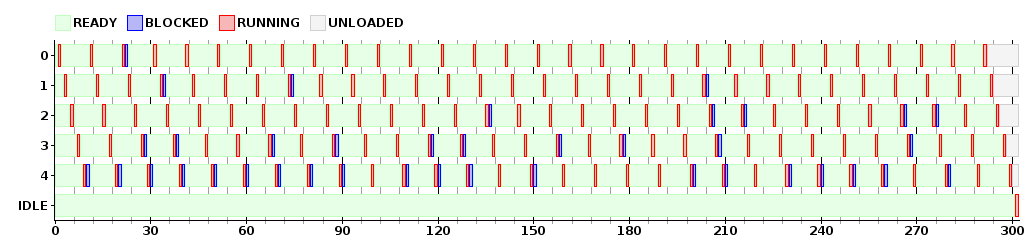
\includegraphics[width=1\textwidth]{img/SchedRRTest1.png}
    \caption{Salida de simusched con quantum 1.}
\end{figure}

\begin{figure}[H]
  \centering
    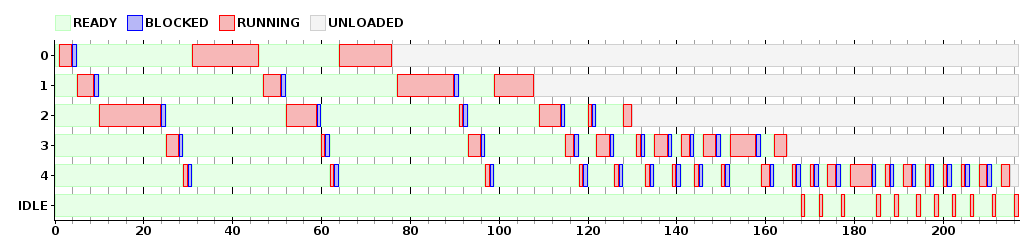
\includegraphics[width=1\textwidth]{img/SchedRRTest15.png}
    \caption{Salida de simusched con quantum 15.}
\end{figure}

Se puede notar que el proceso 2 reci\'en realiza su primer resultado en el ciclo 140 aprox. con quantum 1, mientras que los dem\'as procesos ejecutaron varias veces.\\
Con \quantum 15, solo se ejecuta lo suficiente de cada proceso como para alcanzar su primer IO.

\begin{itemize}
 \item Latencia Promedio $(q=1)$: $(22+34+136+28+10)/5 = 46$
 \item Latencia Promedio $(q=15)$: $(4 + 9 + 24 + 28 + 30) / 5 = 19$
\end{itemize}

\subsection{Tiempo entre ``Respuestas'' }

Quer\'iamos alguna medida que nos lograra orientar sobre el tiempo entre respuesta y respuesta de las tareas Batch. Y lo que hicimos fue medir el tiempo entre cada E/S (Si asumimos que cada IO representa una ``salida'').

\begin{figure}[H]
  \centering
    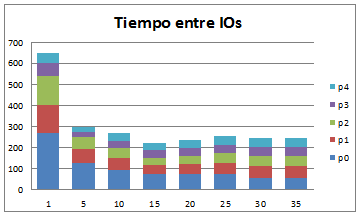
\includegraphics{img/tiempoEntreIOs.png}
    \caption{Gr\'afico comparativo de Tiempo entre IOs para distintos quantums.}
\end{figure}

Se puede observar que al comienzo (como siempre) afecta mucho el tiempo de \cs, y que luego va estabilizandose a partir de un quantum mayor a 10.

\subsection{Llego el momento de decidir... }

Primero vale aclarar que medir con \quantum mayor a 30 no ten\'ia sentido (ya que se tratar\'ia completamente de un scheduler FCFS pues se tendr\'ian \quantums mayores al tiempo total de ejecuci\'on del proceso). Solo los dejamos para mostrar la estabilizaci\'on de las mediciones.

Veamos los resultados que obtuvimos para cada medida:

\begin{description}
 \item[Turnaround] Resultados cercanos al \'optimo entre $q=15$ y $q=35$
 \item[Waiting-Time] Resultados cercanos al \'optimo entre $q=15$ y $q=35$
 \item[Latencia] Resultado \'optimo a partir desde $q=15$
 \item[Tiempo entre IOs] Tiempo entre IOs bueno entre $q=10$ y $q=35$ y el resultado \'optimo en $q=15$
\end{description}

Concluimos que para los casos en los que se trabaja con tareas Batch, de los que solo importa el resultado final, lo que m\'as conviene es utilizar un \quantum que maximize el turnaround ($q=30$ en adelante). Pero este scheduler ser\'ia completamente FCFS con desalojo, por lo que convendr\'ia no utilizar \rr.

Si en cambio se quieren resultados intermedios, debemos tener en cuenta medidas como la latencia y el tiempo entre IOs. Como lo demuestran los resultados, con \quantum 15, tanto para el \ta, \wt, \latencia y el tiempo entre IOs los resultados son buenos.

\newpage

\section{Ejercicio 8}

\subsection{(a) Starvation}

En este algoritmo, es posible que una tarea TaskCPU 20 sufra inanici\'on f\'acilmente en el siguiente esquema:

Procesos:
\begin{itemize}
 \item Una Tarea TaskCPU 20
 \item Dos tareas en el tiempo @1 que esten constantemente haciendo entrada/salida.
\end{itemize}

Colas:
\begin{itemize}
 \item Una cola para procesos interactivos
 \item Una cola para procesos con mucha carga de CPU
\end{itemize}

Archivo de procesos:

\begin{framed}
\begin{verbatim}
# FILE ejercicio8_a.tsk
TaskCPU 20
@1
*2 TaskIOMultiple 20
\end{verbatim}
\end{framed}

Invocaci\'on:

\begin{framed}
\begin{verbatimtab}
./simusched ejercicio8_a.tsk 1 SchedMFQ 2 5 | python \
    graphsched.py > ejercicio8_a.png
\end{verbatimtab}
\end{framed}

\begin{figure}[H]
  \centering
    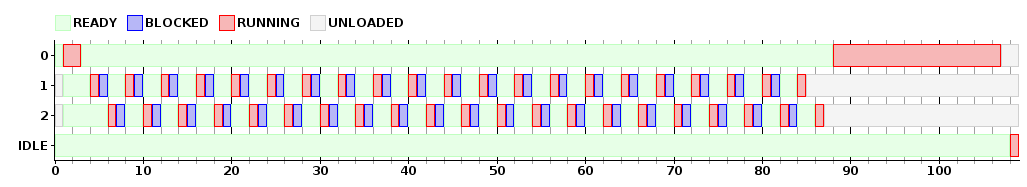
\includegraphics[width=1\textwidth]{img/ejercicio8_a.png}
    \caption{Ejemplo de Inanici\'on.}
\end{figure}

\subsection{(b) Ejemplo de Multicolas}

Ac\'a generamos un ejemplo con tres tareas, cada una con un tipo de comportamiento diferente.

\begin{itemize}
 \item Una tarea de uso intensivo de CPU (TaskCPU 60)
 \item Una tarea de tipo Batch con relativamente poca entrada/salida (TaskBatch 50 3)
 \item Una tarea de tipo cliente interactiva, simulada por una tarea que hace constantemente IO (TaskIOMultiple 15)
\end{itemize}

Luego ejecutamos los tres procesos en un scheduler MFQ con tres colas de pioridad (2 5 10)

\begin{framed}
\begin{verbatim}
# FILE ejercicio8_b.tsk
TaskCPU 60             # p0
TaskBatch 50 3         # p1
TaskIOMultiple 15      # p2
\end{verbatim}
\end{framed}

Invocaci\'on:

\begin{framed}
\begin{verbatim}
./simusched ejercicio8_b.tsk 1 SchedMFQ 2 5 10 | python \
      graphsched.py > ejercicio8_b.png
\end{verbatim}
\end{framed}

El resultado fue el siguiente:

\begin{figure}[H]
  \centering
    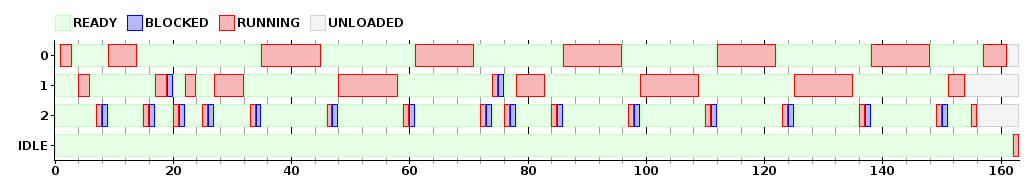
\includegraphics[width=1\textwidth]{img/ejercicio8_b.png}
    \caption{Ejemplo de MFQ}
\end{figure}

En el gr\'afico se puede ver como los procesos van cambiando de cola de pioridad. En un principio las tres tareas comienzan ejecutandose en la cola de mayor prioridad. Se puede ver que como el proceso p0 (0) consume siempre su \quantum sin bloquearse  y de esta manera va perdiendo su prioridad, es decir va cambiando a una cola de menor prioridad, y por lo tanto ejecutandose durante m\'as tiempo cada vez que lo hace, pero con una menor frecuencia.\\
En cambio, el proceso p2 (2) se mantiene siempre en la prioridad m\'as alta, dado que se bloquea constantemente y nunca alcanza a realizar el \quantum completo. De esta manera el proceso p2 se ejecuta con un \quantum menor pero con una mayor frecuencia.\\
Por \'ultimo el proceso p1 (1) va a ir alternando su prioridad dependiendo si se bloqueo o no durante la ejecuci\'on de su \quantum anterior, esto se puede ver bien en el gr\'afico viendo como var\'ia la cantidad de ciclos en los que esta ejecutandose sin bloquearse, es decir el proceso va alternandose en colas que tienen mayor y menor \quantum.

\end{document}


